\begin{tikzpicture}[transform canvas={scale=0.9}] 
  \begin{scope}[yshift=0.2\textwidth]
    \begin{scope}[xshift=0cm]
      \node [mybox] (all) at (0, 0) {
        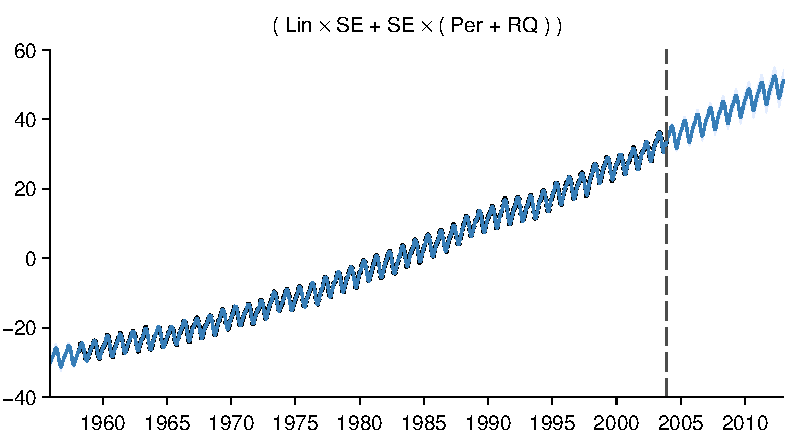
\includegraphics[width=0.8\textwidth, height=0.3\textwidth]{figures/03-mauna2003-s_all.pdf}
      };
    \end{scope}
  \end{scope}
  \begin{scope}[yshift=0\textwidth]
    \begin{scope}[xshift=0cm]
    \end{scope}
  \end{scope}
  \begin{scope}[yshift=0.27\textwidth]
    \begin{scope}[xshift=5cm]
        \node [mybox, below of=all] (equals) at (0, 0) {\Huge{$=$}};
    \end{scope}
  \end{scope}
  \begin{scope}[yshift=-0.1\textwidth]
    \begin{scope}[xshift=-0.3\textwidth]
      \node [mybox] (all) at (0, 0) {
        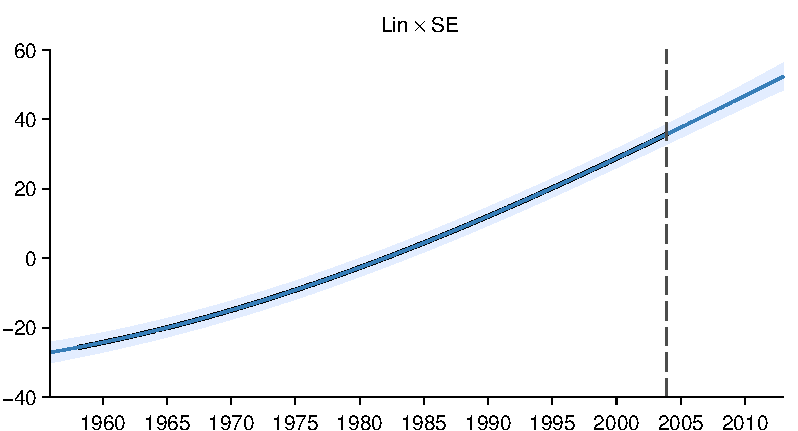
\includegraphics[width=0.5\textwidth]{figures/03-mauna2003-s_1.pdf}
      };
    \end{scope}
    \begin{scope}[xshift=+0.3\textwidth]
      \node [mybox] (all) at (0, 0) {
        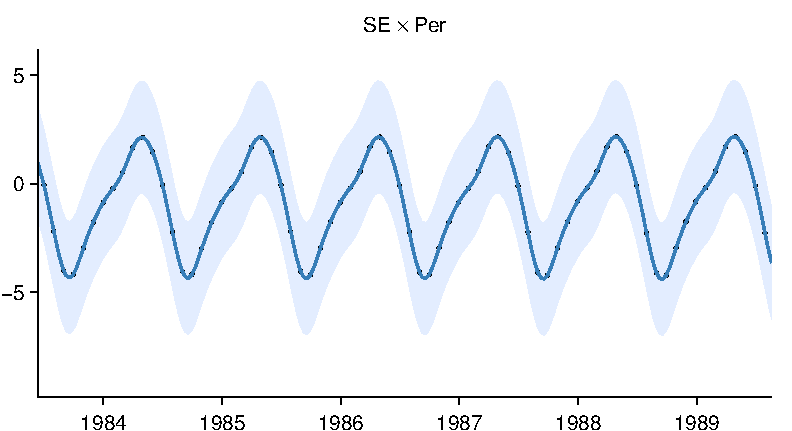
\includegraphics[width=0.5\textwidth]{figures/03-mauna2003-s_2_zoom.pdf}
      };
    \end{scope}
  \end{scope}
  \begin{scope}[yshift=-0.15\textwidth]
    \begin{scope}[xshift=0cm]
        \node [mybox, below of=all] (equals) at (0, 0) {\Huge{+}};
    \end{scope}
  \end{scope}
  \begin{scope}[yshift=-0.35\textwidth]
    \begin{scope}[xshift=-0.3\textwidth]
      \node [mybox] (all) at (0, 0) {
        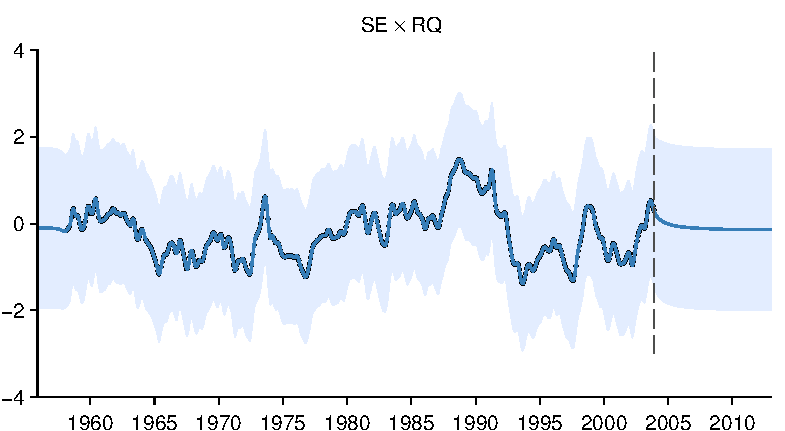
\includegraphics[width=0.5\textwidth]{figures/03-mauna2003-s_3.pdf}
      };
    \end{scope}
    \begin{scope}[xshift=+0.3\textwidth]
      \node [mybox] (all) at (0, 0) {
        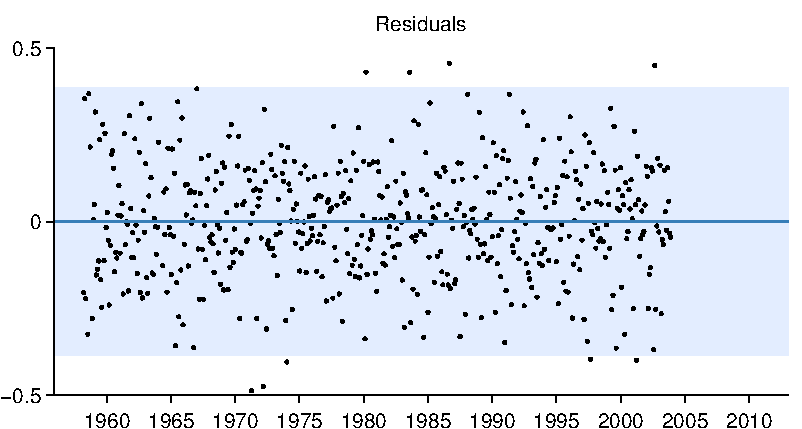
\includegraphics[width=0.5\textwidth]{figures/03-mauna2003-s_resid.pdf}
      };
    \end{scope}
  \end{scope}
\end{tikzpicture}
